\section{Résultats de l'analyse sur l'outil}\label{sec:analyse_stationnement}
L'outil d'analyse a été utilisé pour créer un inventaire de stationnement. Cette section donnera des détails sur les résultats obtenus en 4 parties. Premièrement, les résultats de la méthode de calcul automatique seront discutés. Dans un deuxième temps, un exemple de calcul de validation sera montré. En troisième lieu, les modifications faites de manière semi automatique ou manuelle seront détaillées et discutées. Finalement, des exemples d'analyses possibles seront montrés à titre indicatif. 

\subsection{Résultats du calcul automatique}
L'inventaire automatique a été calculé pour l'ensemble des propriétés dans les limites de la ville de Québec. Ces calculs ont initialement été faits via un script Python indépendant puis manipulés à l'aide de l'interface développé.  Dans cette section, l'inventaire sera dressé en utilisant les minimums calculés sauf indication contraire. Au total, la méthode réglementaire donne un estimé de 498 800 places de stationnement. La figure \ref{fig:result-dist-places-par-usage} montre la distribution des places de stationnement entre les différents usages du sol.\par
\begin{figure}[!h]
    \centering
    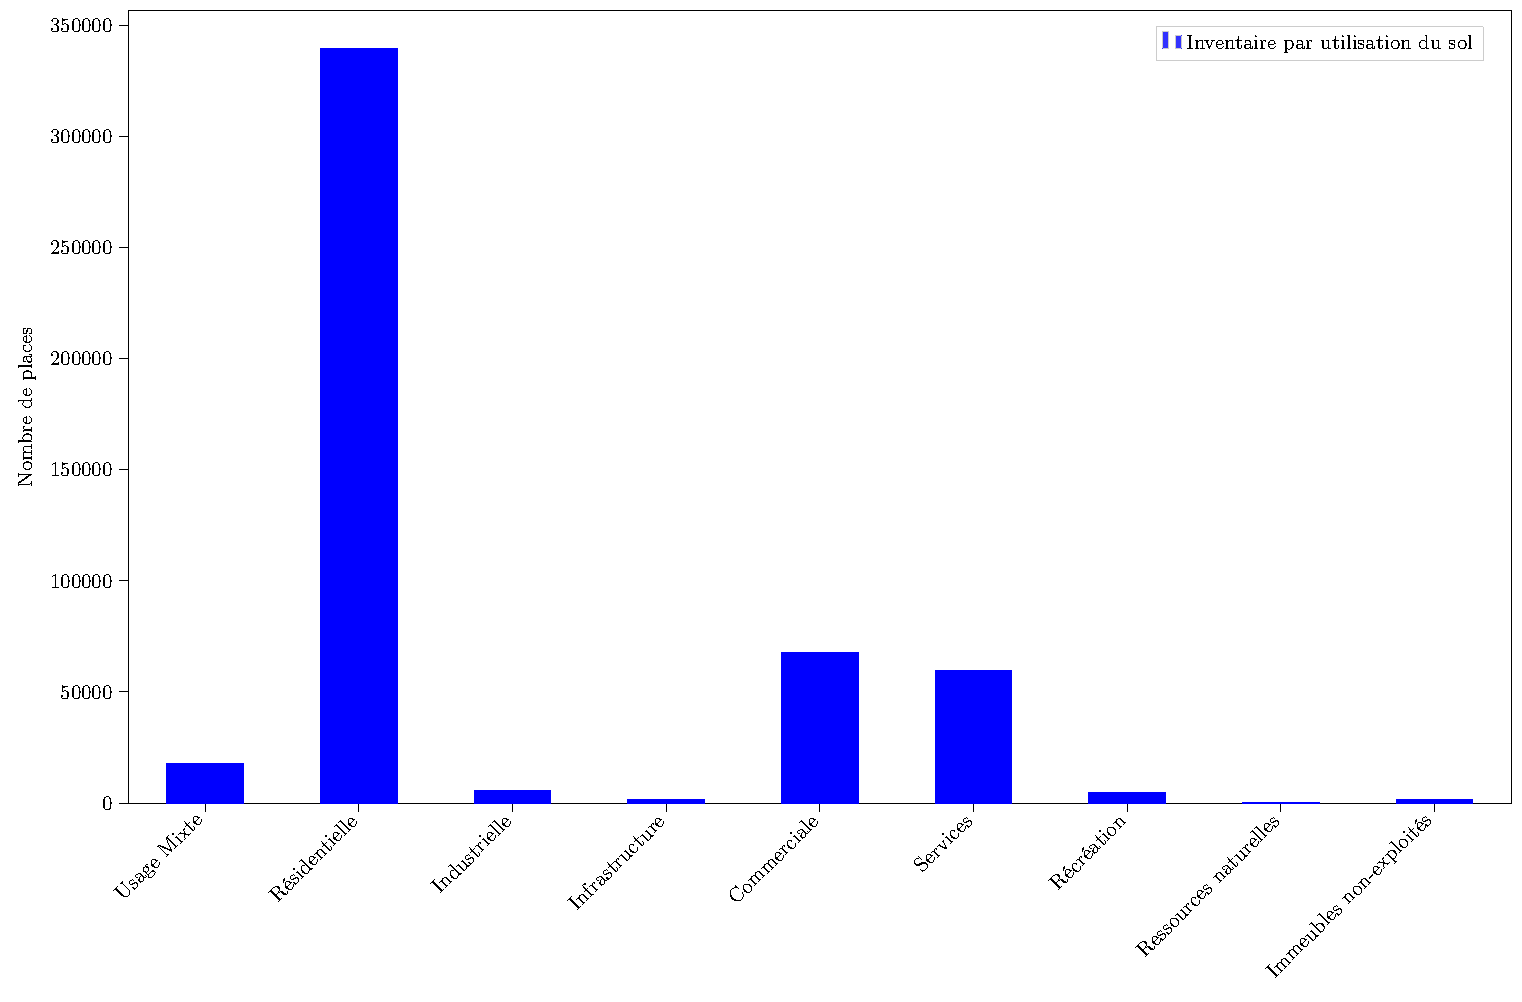
\includegraphics[width=1\textwidth]{figures/inventaire-reg-par-cubf.pdf}
    \caption{Distribution des places des stationnements par utilisation du sol}
    \label{fig:result-dist-places-par-usage}
\end{figure}
On constate que les stationnement résidentiels (305 700 places) constituent 65\% du parc de stationnement hors-rue. Même en prenant compte du plus fort taux de données absentes dans les propriétés commerciales (67 000 places de stationnement) et de services(58 800 places de stationnement) (environ 30 à 45\% de données manquantes). Le stationnement résidentiel demeurerait le contributeur majeur au parc total. \par 
\FloatBarrier
Ce parc de stationnement n'est pas uniformément réparti sur le territoire. Les figure \ref{fig:result-dist-places-par-quartier} et \ref{fig:n-places-reg-carto} montrent la distribution spatiale du parc de stationnement dans la ville de Québec selon les quartiers administratifs. On constate que les secteurs Duberger-Les Saules et Neufchatel-Est et la Cité Universitaire contiennent une grande partie du parc de stationnement hors-rue. 
\begin{figure}[h]
    \centering
    \begin{subfigure}[b]{0.9\textwidth}
        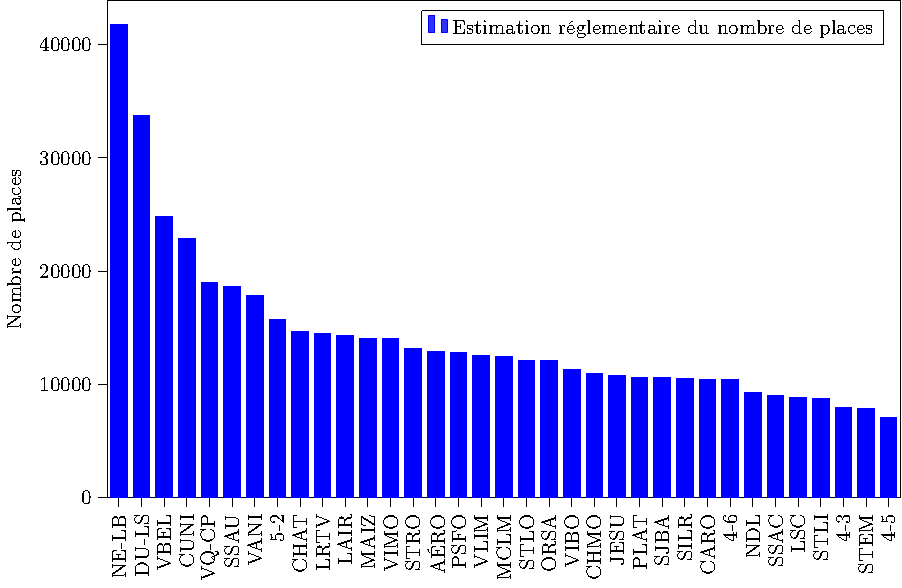
\includegraphics[width=1\textwidth]{figures/inventaire-reg-par-quartier.pdf}
        \caption{Histogramme}
        \label{fig:result-dist-places-par-quartier}
    \end{subfigure}
    ~
    \begin{subfigure}[b]{0.9\textwidth}
        \centering
        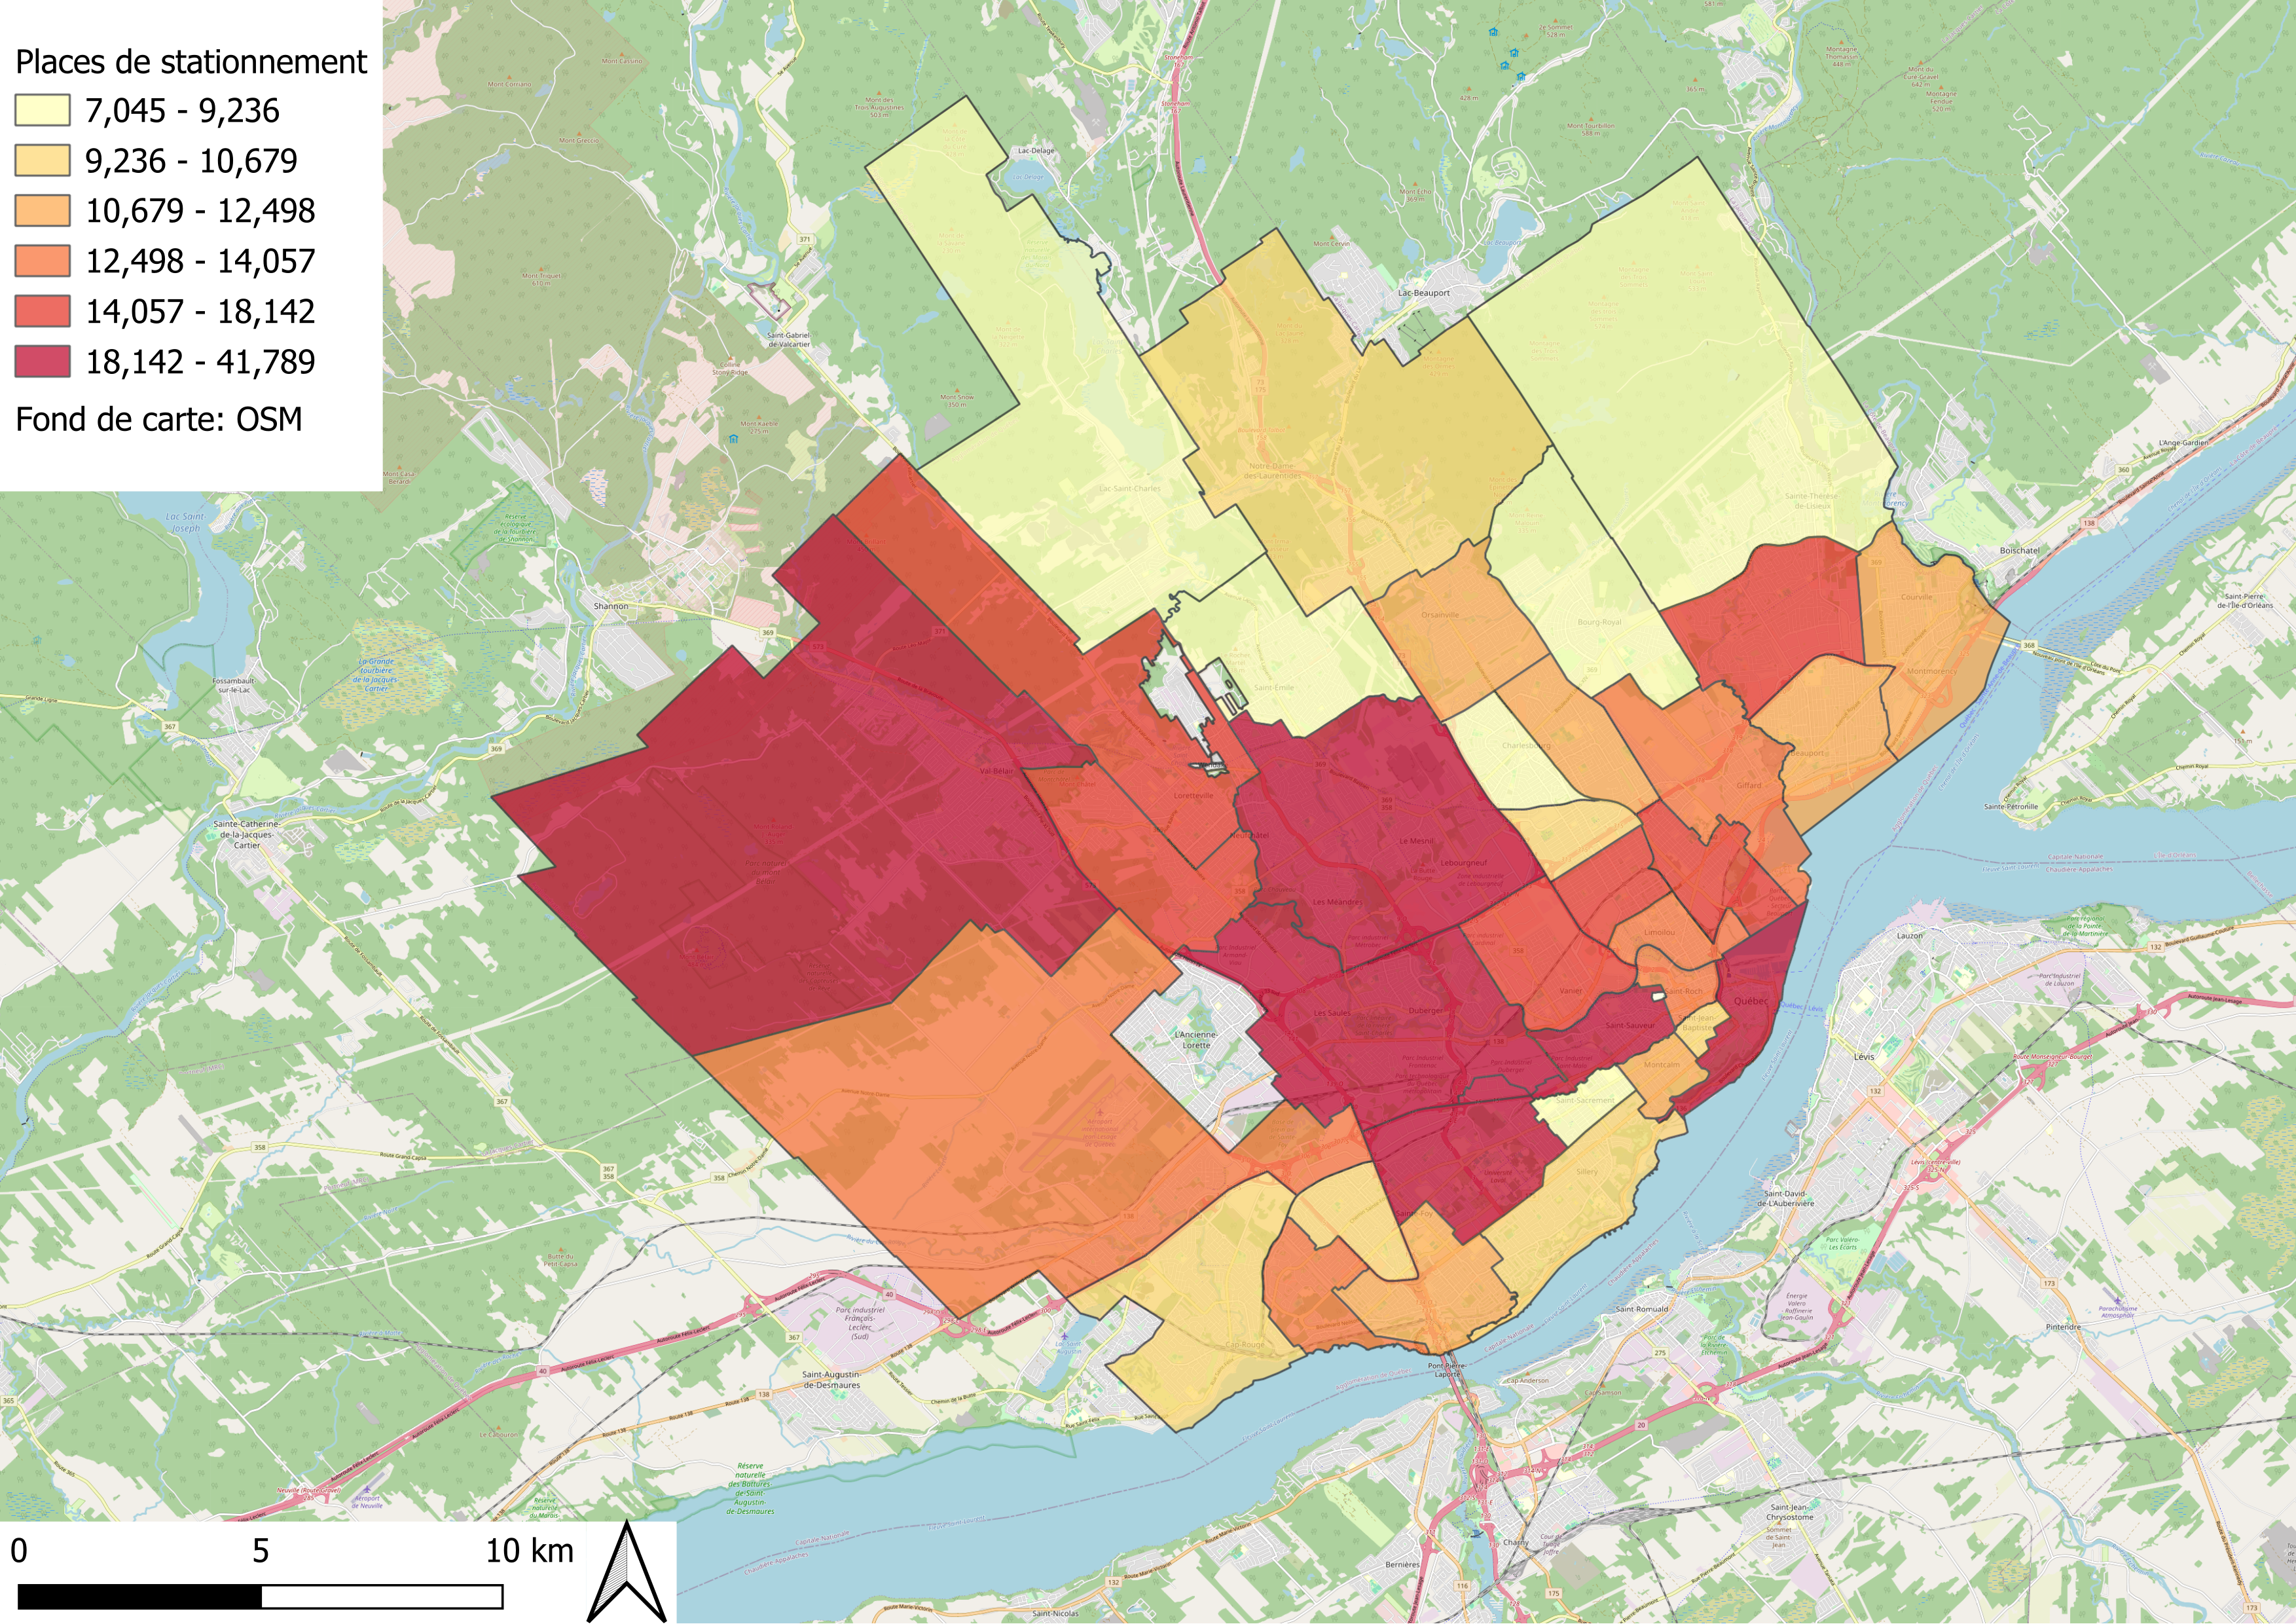
\includegraphics[width=1\linewidth]{images/n-places-reg.png}
        \caption{Carte}
        \label{fig:n-places-reg-carto}
    \end{subfigure}
    \caption{Distribution des places de stationnement sur le territoire}
\end{figure}
\FloatBarrier
La densité de stationnement suit essentiellement le même schéma que la densité de population comme le montrent les figures \ref{fig:dens-pop} et \ref{fig:dens-stat}.
\begin{figure}[!h]
    \centering
    \begin{subfigure}[b]{0.725\textwidth}
        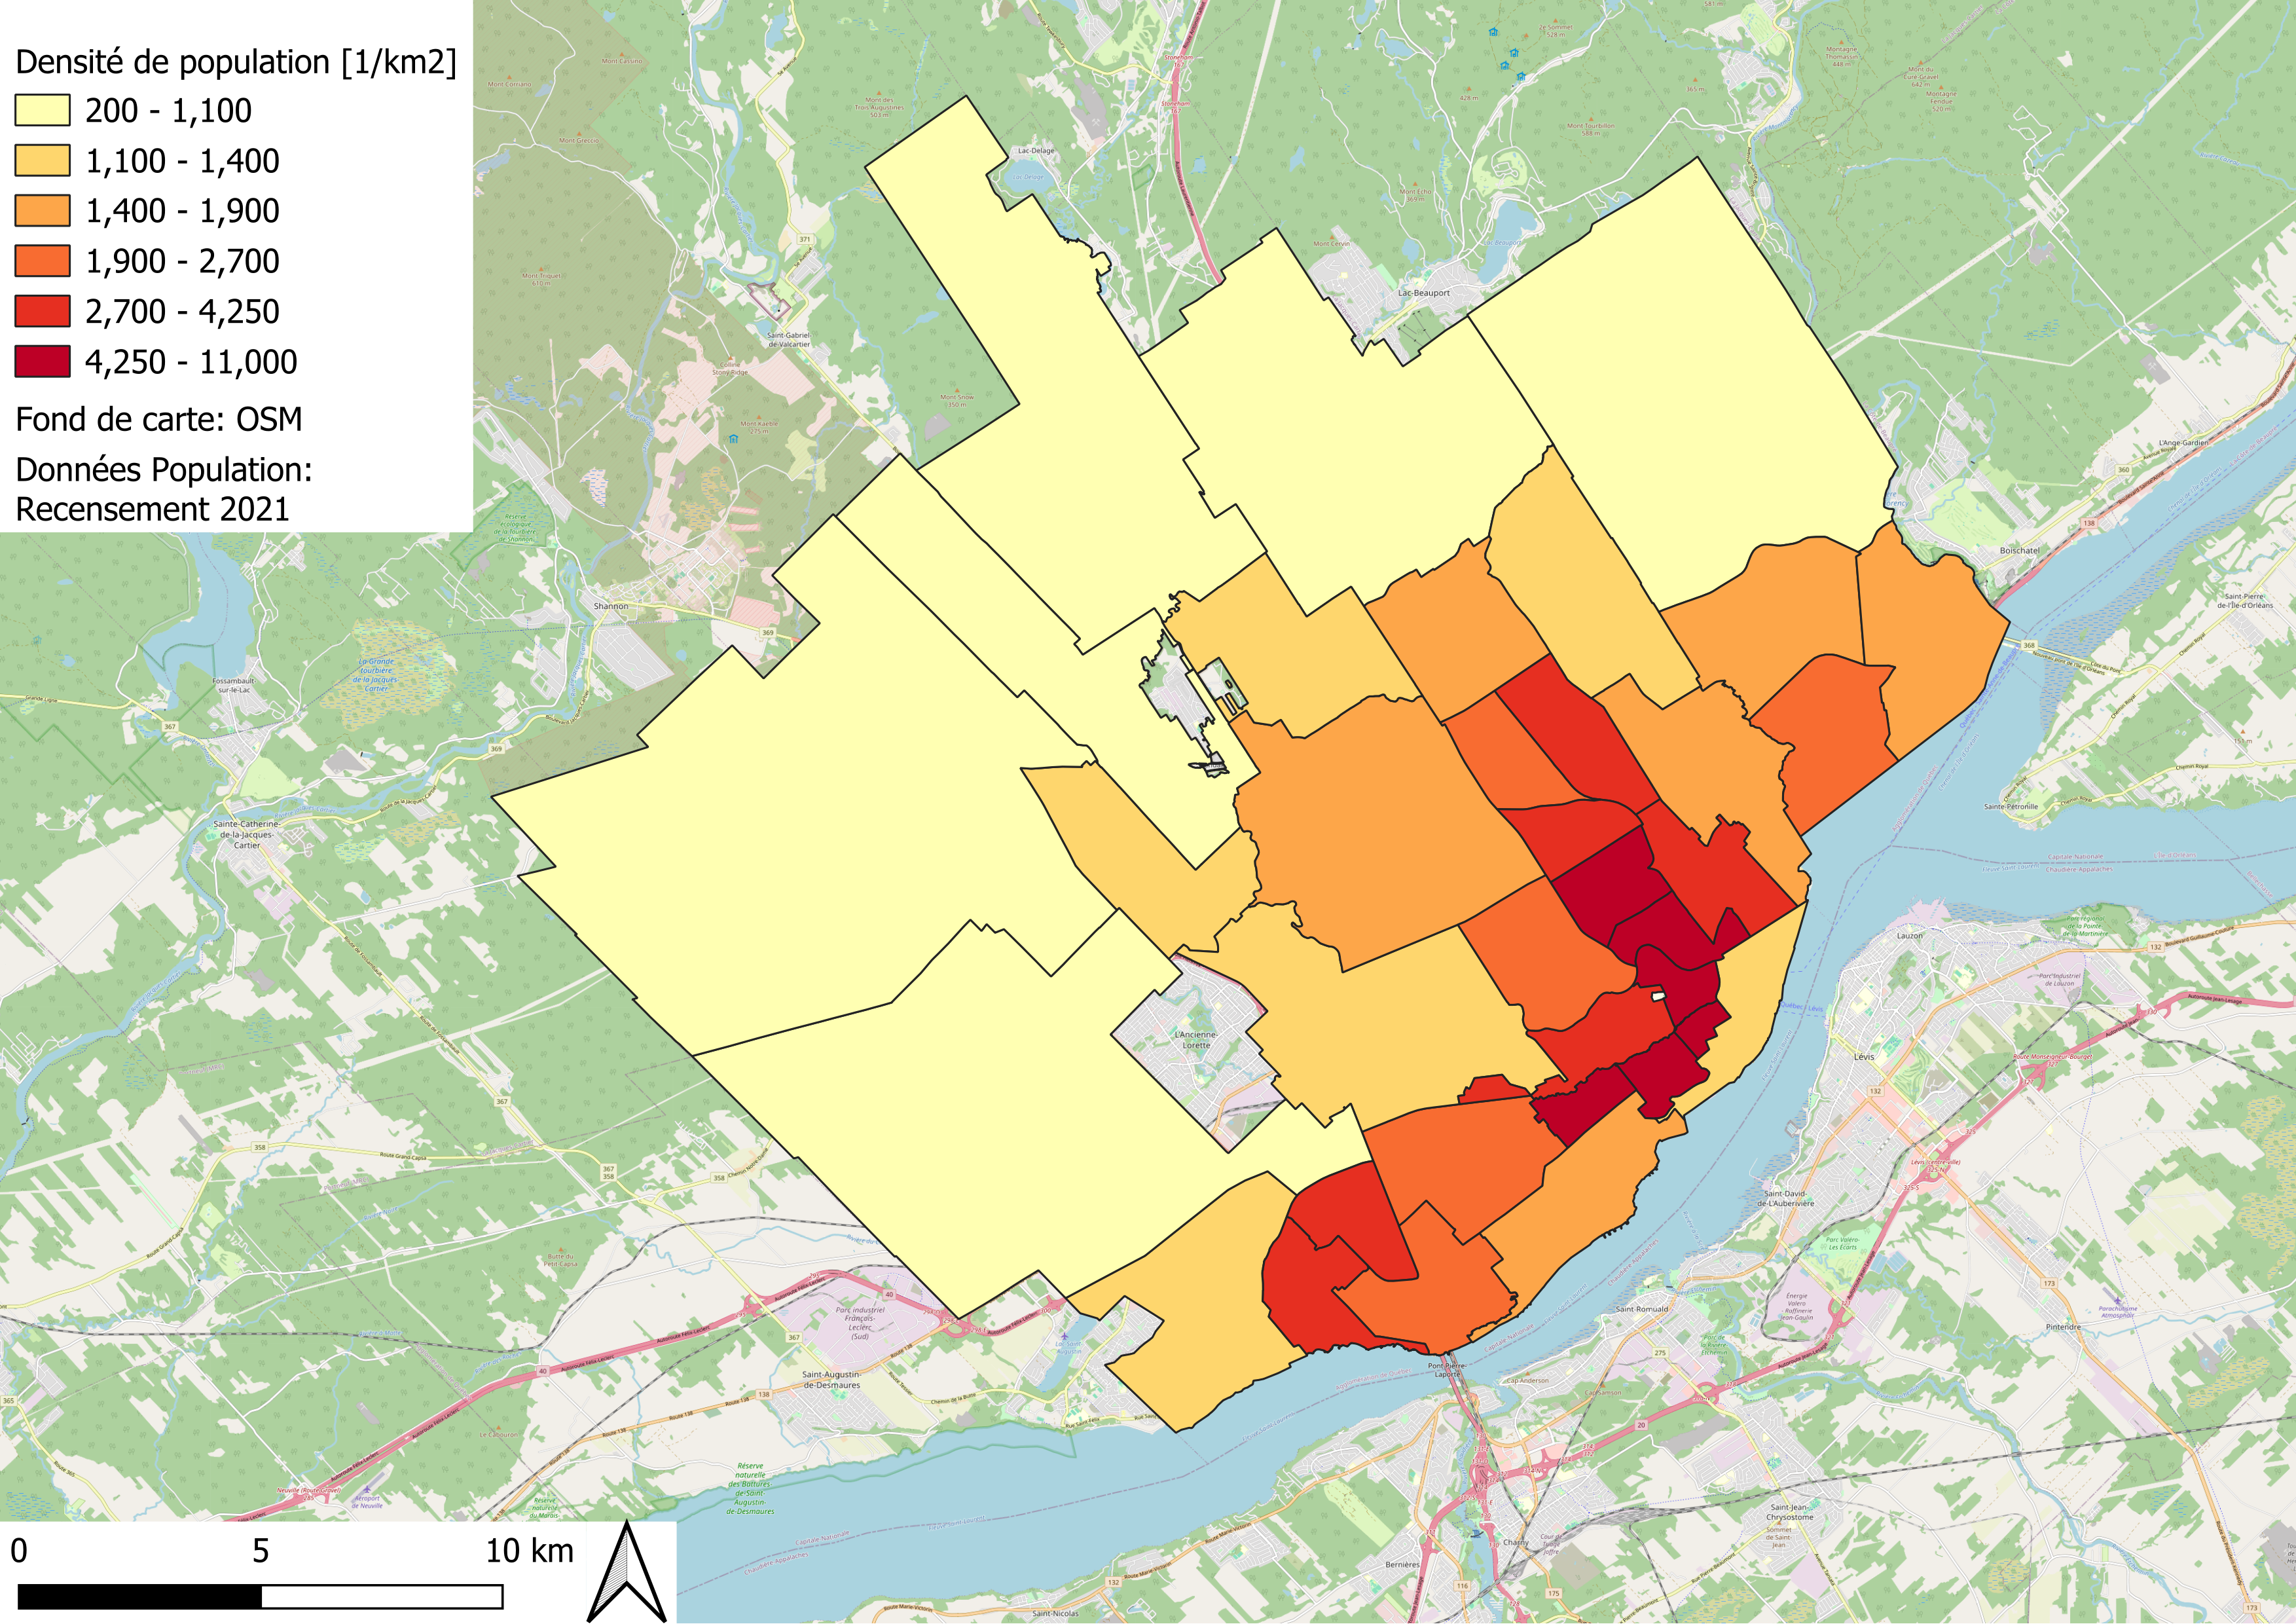
\includegraphics[width=1\textwidth]{images/densite-pop.png}
        \caption{Population}
        \label{fig:dens-pop}
    \end{subfigure}
    ~
    \begin{subfigure}[b]{0.725\textwidth}
        \centering
        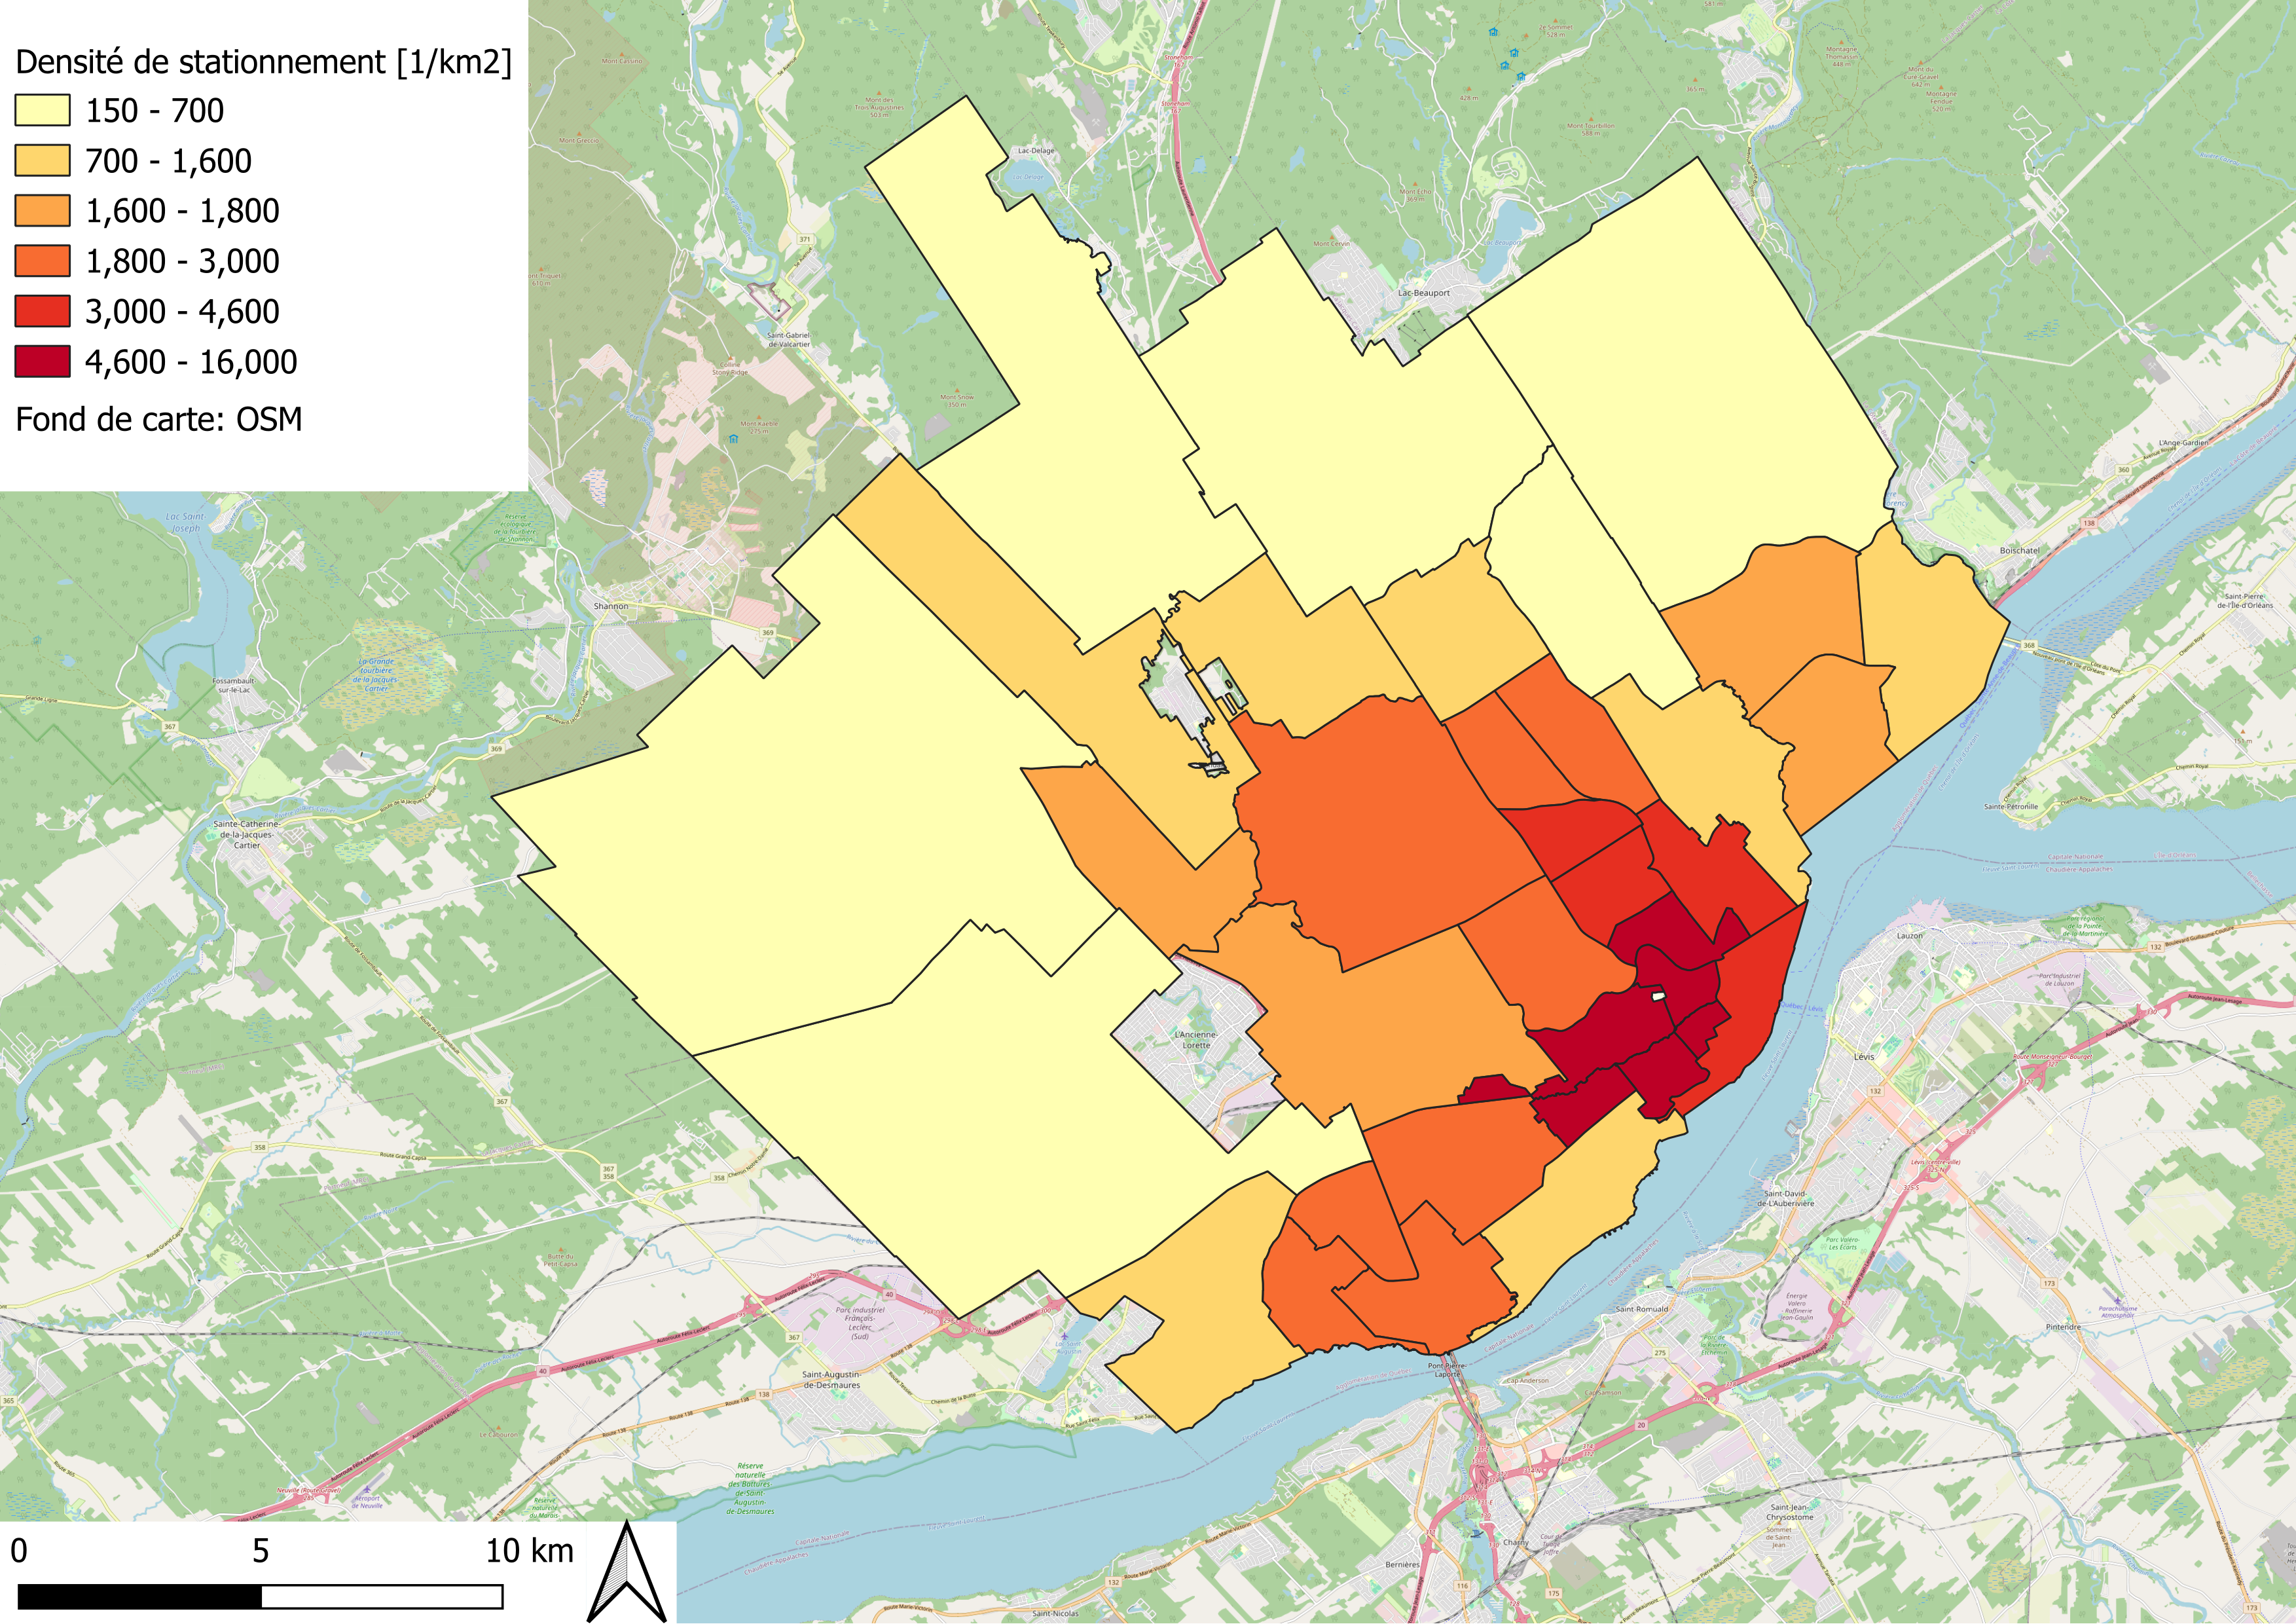
\includegraphics[width=1\linewidth]{images/densite-stat-reg.png}
        \caption{Stationnement}
        \label{fig:dens-stat}
    \end{subfigure}
    \caption{Distribution de la densité de stationnement et de population sur le territoire}
\end{figure}\FloatBarrier
La distribution de la capacité de stationnement entre les différentes utilisation du sol n'est pas la même selon les quartiers comme le montre la figure \ref{fig:dist-stat-quart-util}.\par

\begin{figure}[!h]
    \centering
    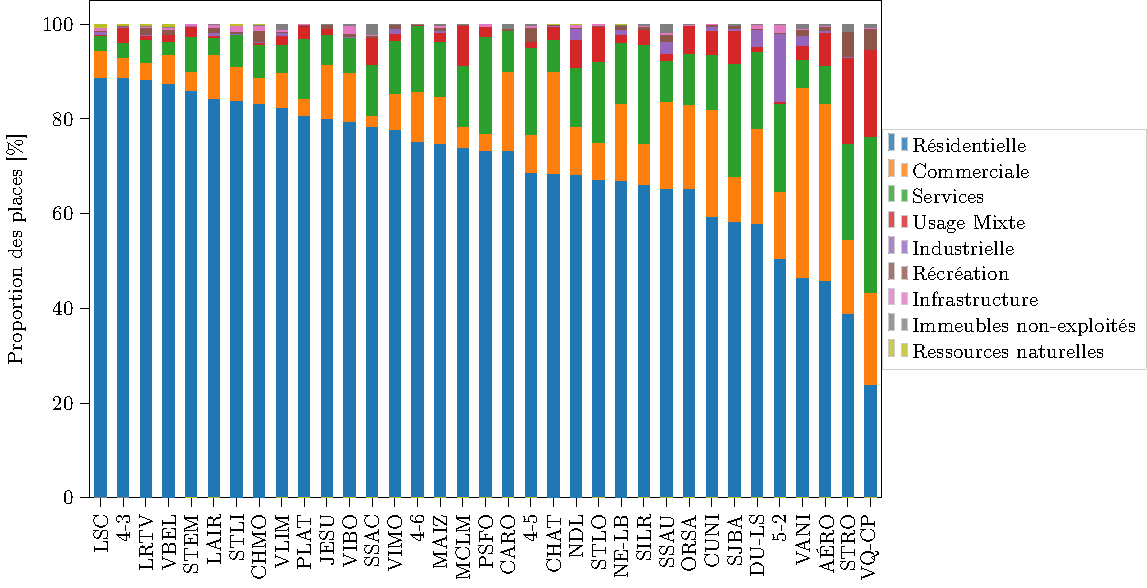
\includegraphics[width=1\linewidth]{figures/distr-inv-prop-quart-util.pdf}
    \caption{Distribution du nombre de places par quartier et usage du sol}
    \label{fig:dist-stat-quart-util}
\end{figure}
\subsection{Évaluation du modèle de prédiction}\label{ssec:eval-park-pred-perf}
Cette section fera des constats sur l'échantillonnage effectué pour informer sur la précision des estimés faits dans la section précédente. Chaque strate aura une section où seront discutés les constats sur la strate en particulier et les conséquences des erreurs mesurées sur l'inventaire total. Le tableau \ref{tab:confidence-interval-parking-supply} montre le résultat des calculs d'intervalle de confiance
\begin{table}[h]
    \centering
    \caption{Sommaire des intervalles de confiance de l'offre de stationnement ($\alpha=0.05$)}
    \label{tab:confidence-interval-parking-supply}
    \begin{tabular}{llllll}
        \hline
        Strate                  & N     & n     & $S_{predit}$  & $S_{inf}$    & $S_{sup}$  \\ \hline
        Logement unifamilial    & 97748 & 30    & 130100        & 88394         & 189400        \\
        Logement Plex           & 23621 & 30    & 88139         & 58356         & 119003        \\
        Logement Blocs Appart   & 2465  & 30    & 78783         & 67767         & 89953         \\
        Commercial              & 1552  & 29    & 67217         & 55583         & 77689         \\
        Services                & 1623  & 27    & 57803         & 40297         & 71920         \\
        Industriel              & 176   & 26    & 5586          & 3948          & 6873          \\
        Assemblée               & 149   & 23    & 4529          & 785           & 7957          \\
        Usage multiple          & 156   & 17    & 7301          & 1192          & 10443         \\
        \hline
    \end{tabular}
    
\end{table}
\FloatBarrier
\subsubsection{Résidentielle unifamiliale}
Trente propriétés ont été échantillonnées.  La figure \hl{insert} montre la distribution des erreurs 
\subsection{Résultats connexes à l'inventaire}
La motorisation a été estimée ainsi que les profils d'accumulation véhicule à partir des données de l'enquête OD. On peut donc commencer à interroger la mesure dans laquelle le stationnement est saturé. Les figure \ref{fig:places-res-voit-res-hist} et \ref{fig:places-res-voit-res-carte} montrent le nombre de places résidentielles hors-rue par résident. Les résultats montrent qu'il y a plus de places de stationnement par voiture dans les quartier centraux ce qui n'est pas conforme aux attentes puisque les quartiers centraux sont typiquement là où l'on trouve des enjeux de stationnement. Dans un premier temps, on peut penser que la méthode de calcul qui applique les règlements des années '90 pour tous les logements avant 1990 va sur estimer la quantité de stationnement dans les quartiers centraux. D'autre part, on peut penser que les résidences dans les quartiers périphériques auront plus de stationnement que le minimum. 
\begin{figure}
    \centering
    \begin{subfigure}{1\textwidth}
        \centering
        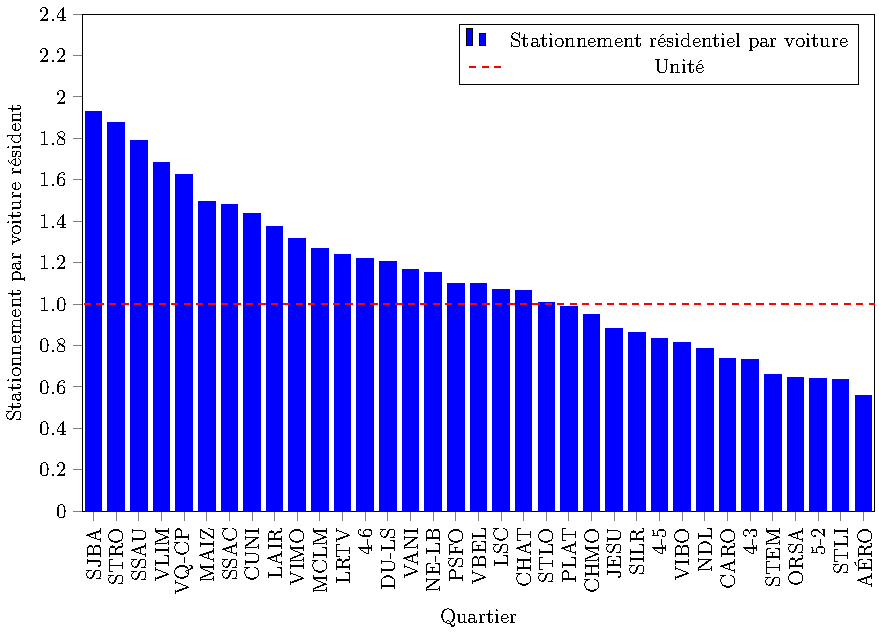
\includegraphics[width=0.75\linewidth]{figures/places-res-par-voit-res.pdf}
        \caption{Histogramme}
        \label{fig:places-res-voit-res-hist}
    \end{subfigure}
    ~
    \begin{subfigure}{1\textwidth}
        \centering
        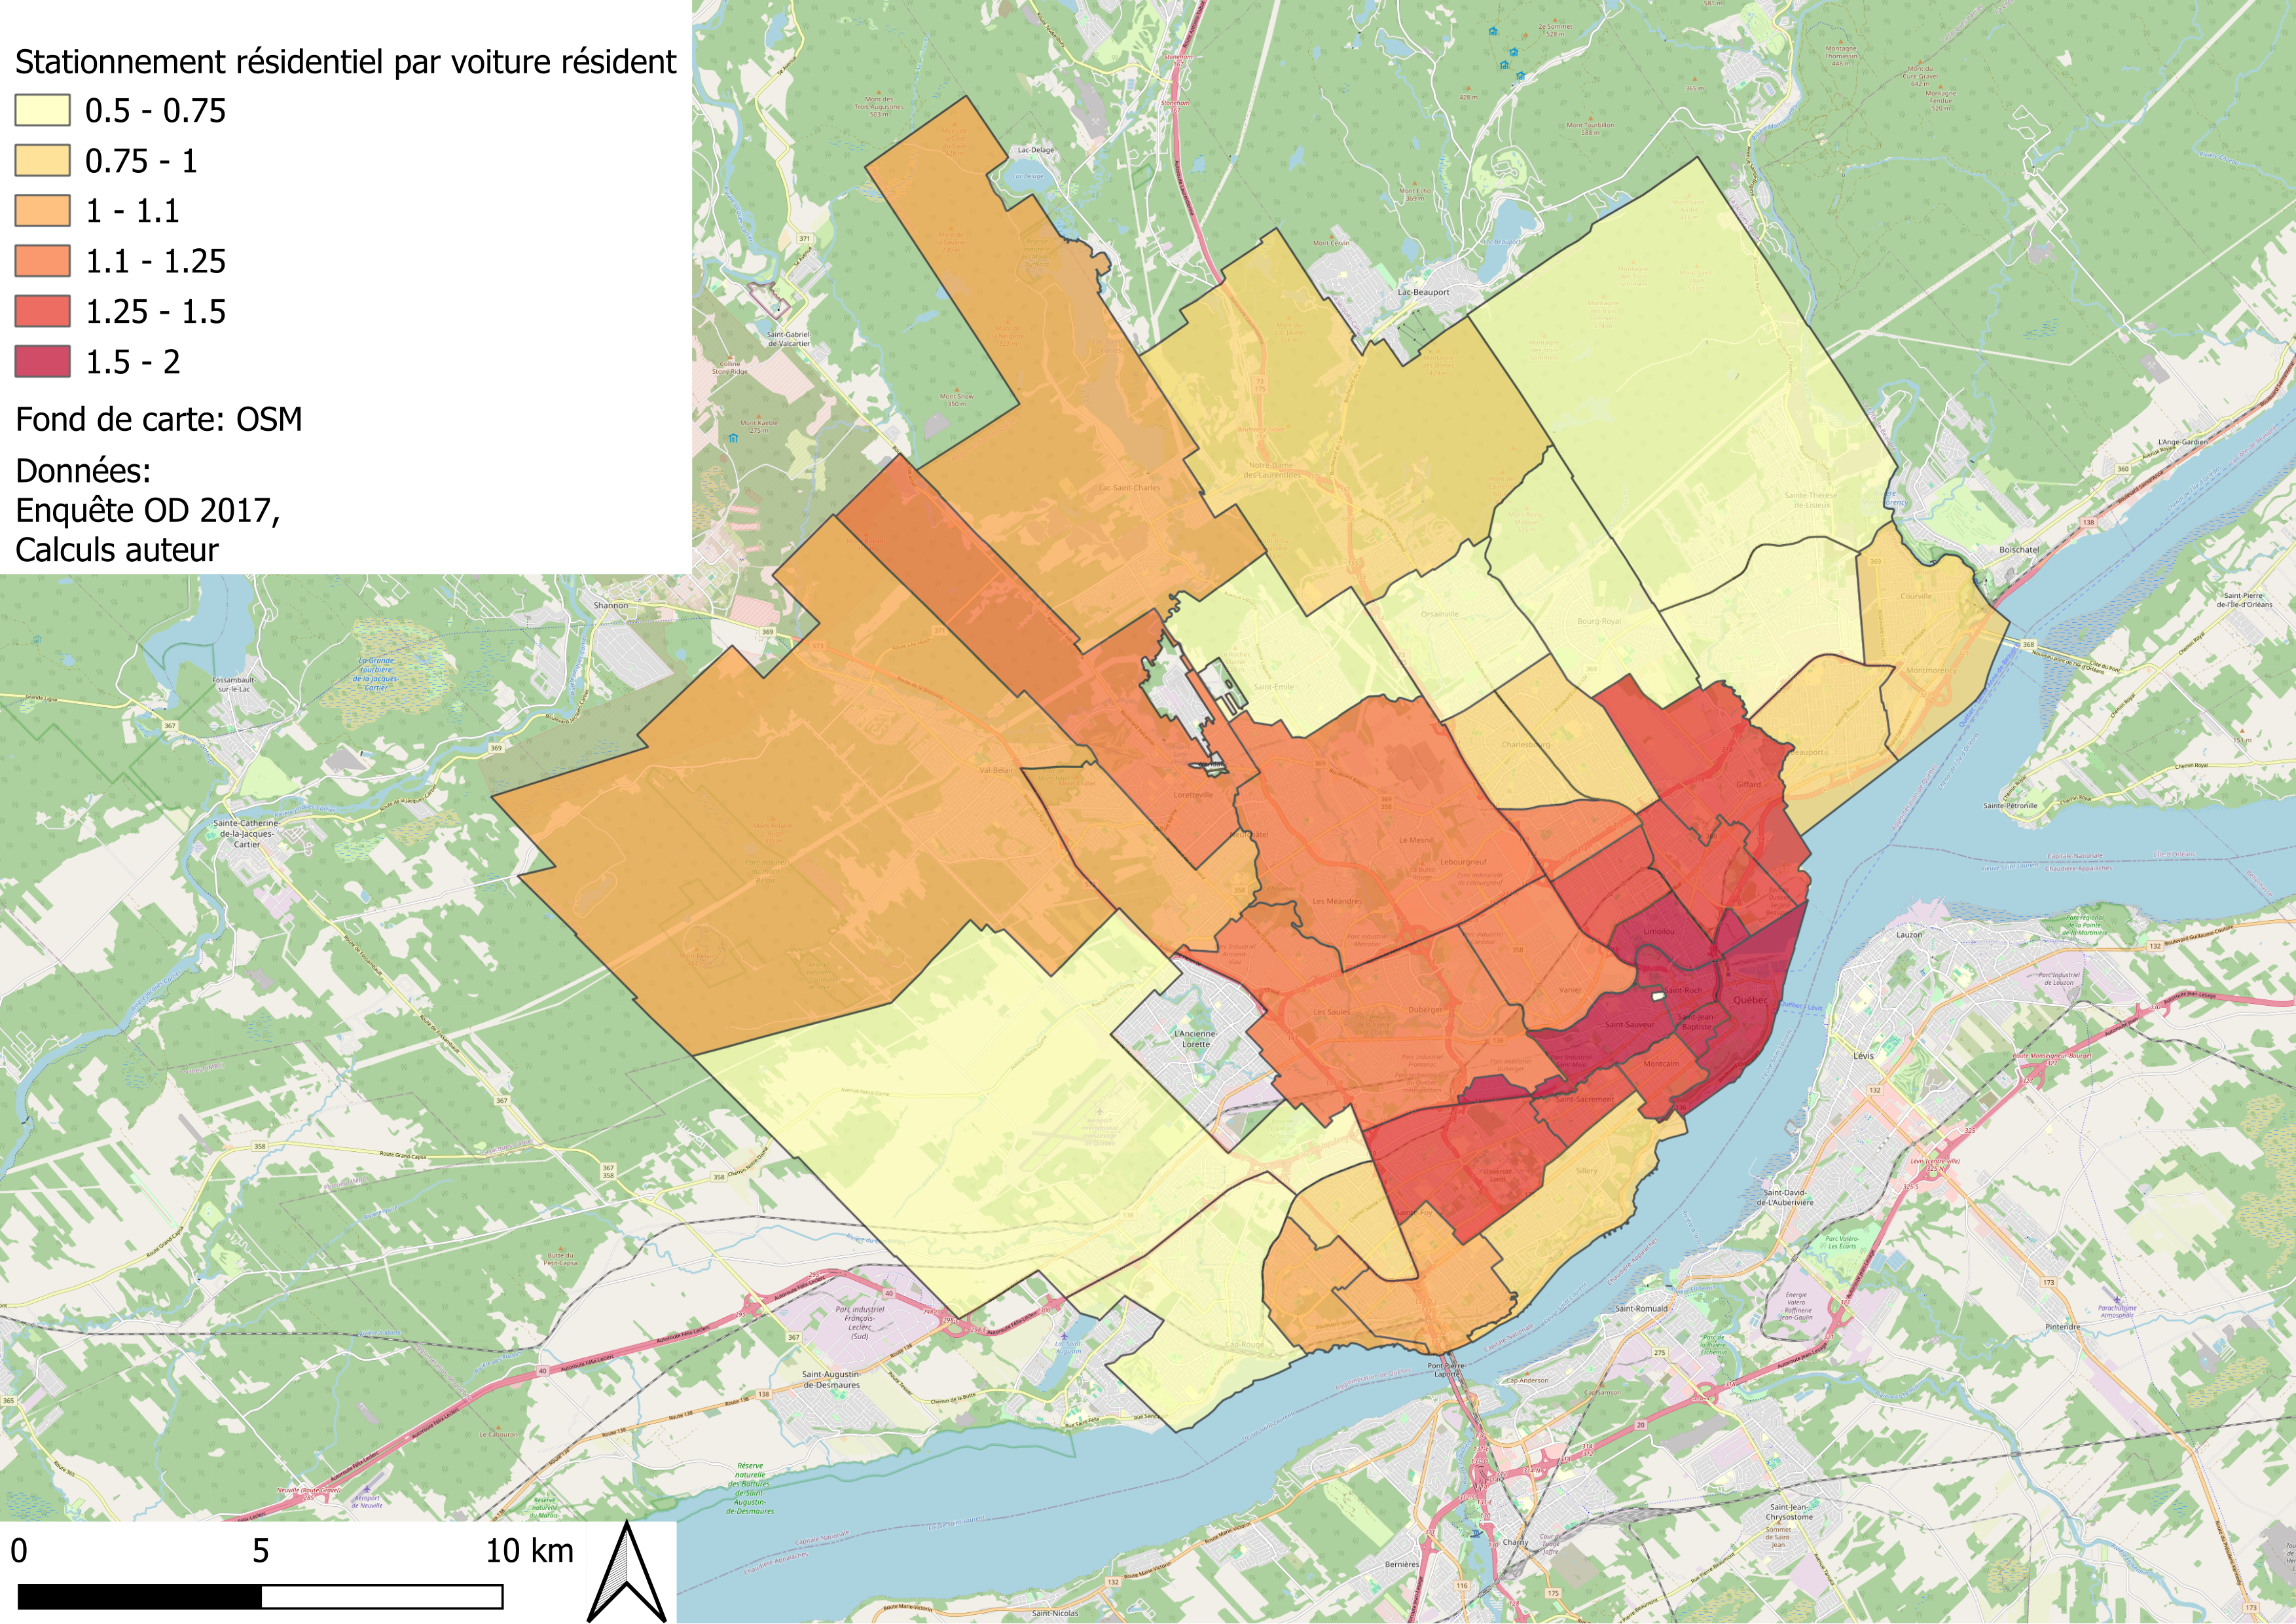
\includegraphics[width=0.75\linewidth]{images/stat-res-par-voit-res.png}
        \caption{Carte}
        \label{fig:places-res-voit-res-carte}
    \end{subfigure}
    \caption{Nombre de places résidentielles par voiture des résidents}
    \label{fig:places-res-voit-res}
\end{figure}
\FloatBarrier
D'autre part, les quartiers centraux ont des taux de motorisation plus faibles comme le montre la figure \ref{fig:motorisation-par-quartier}. 
\begin{figure}[!h]
    \centering
    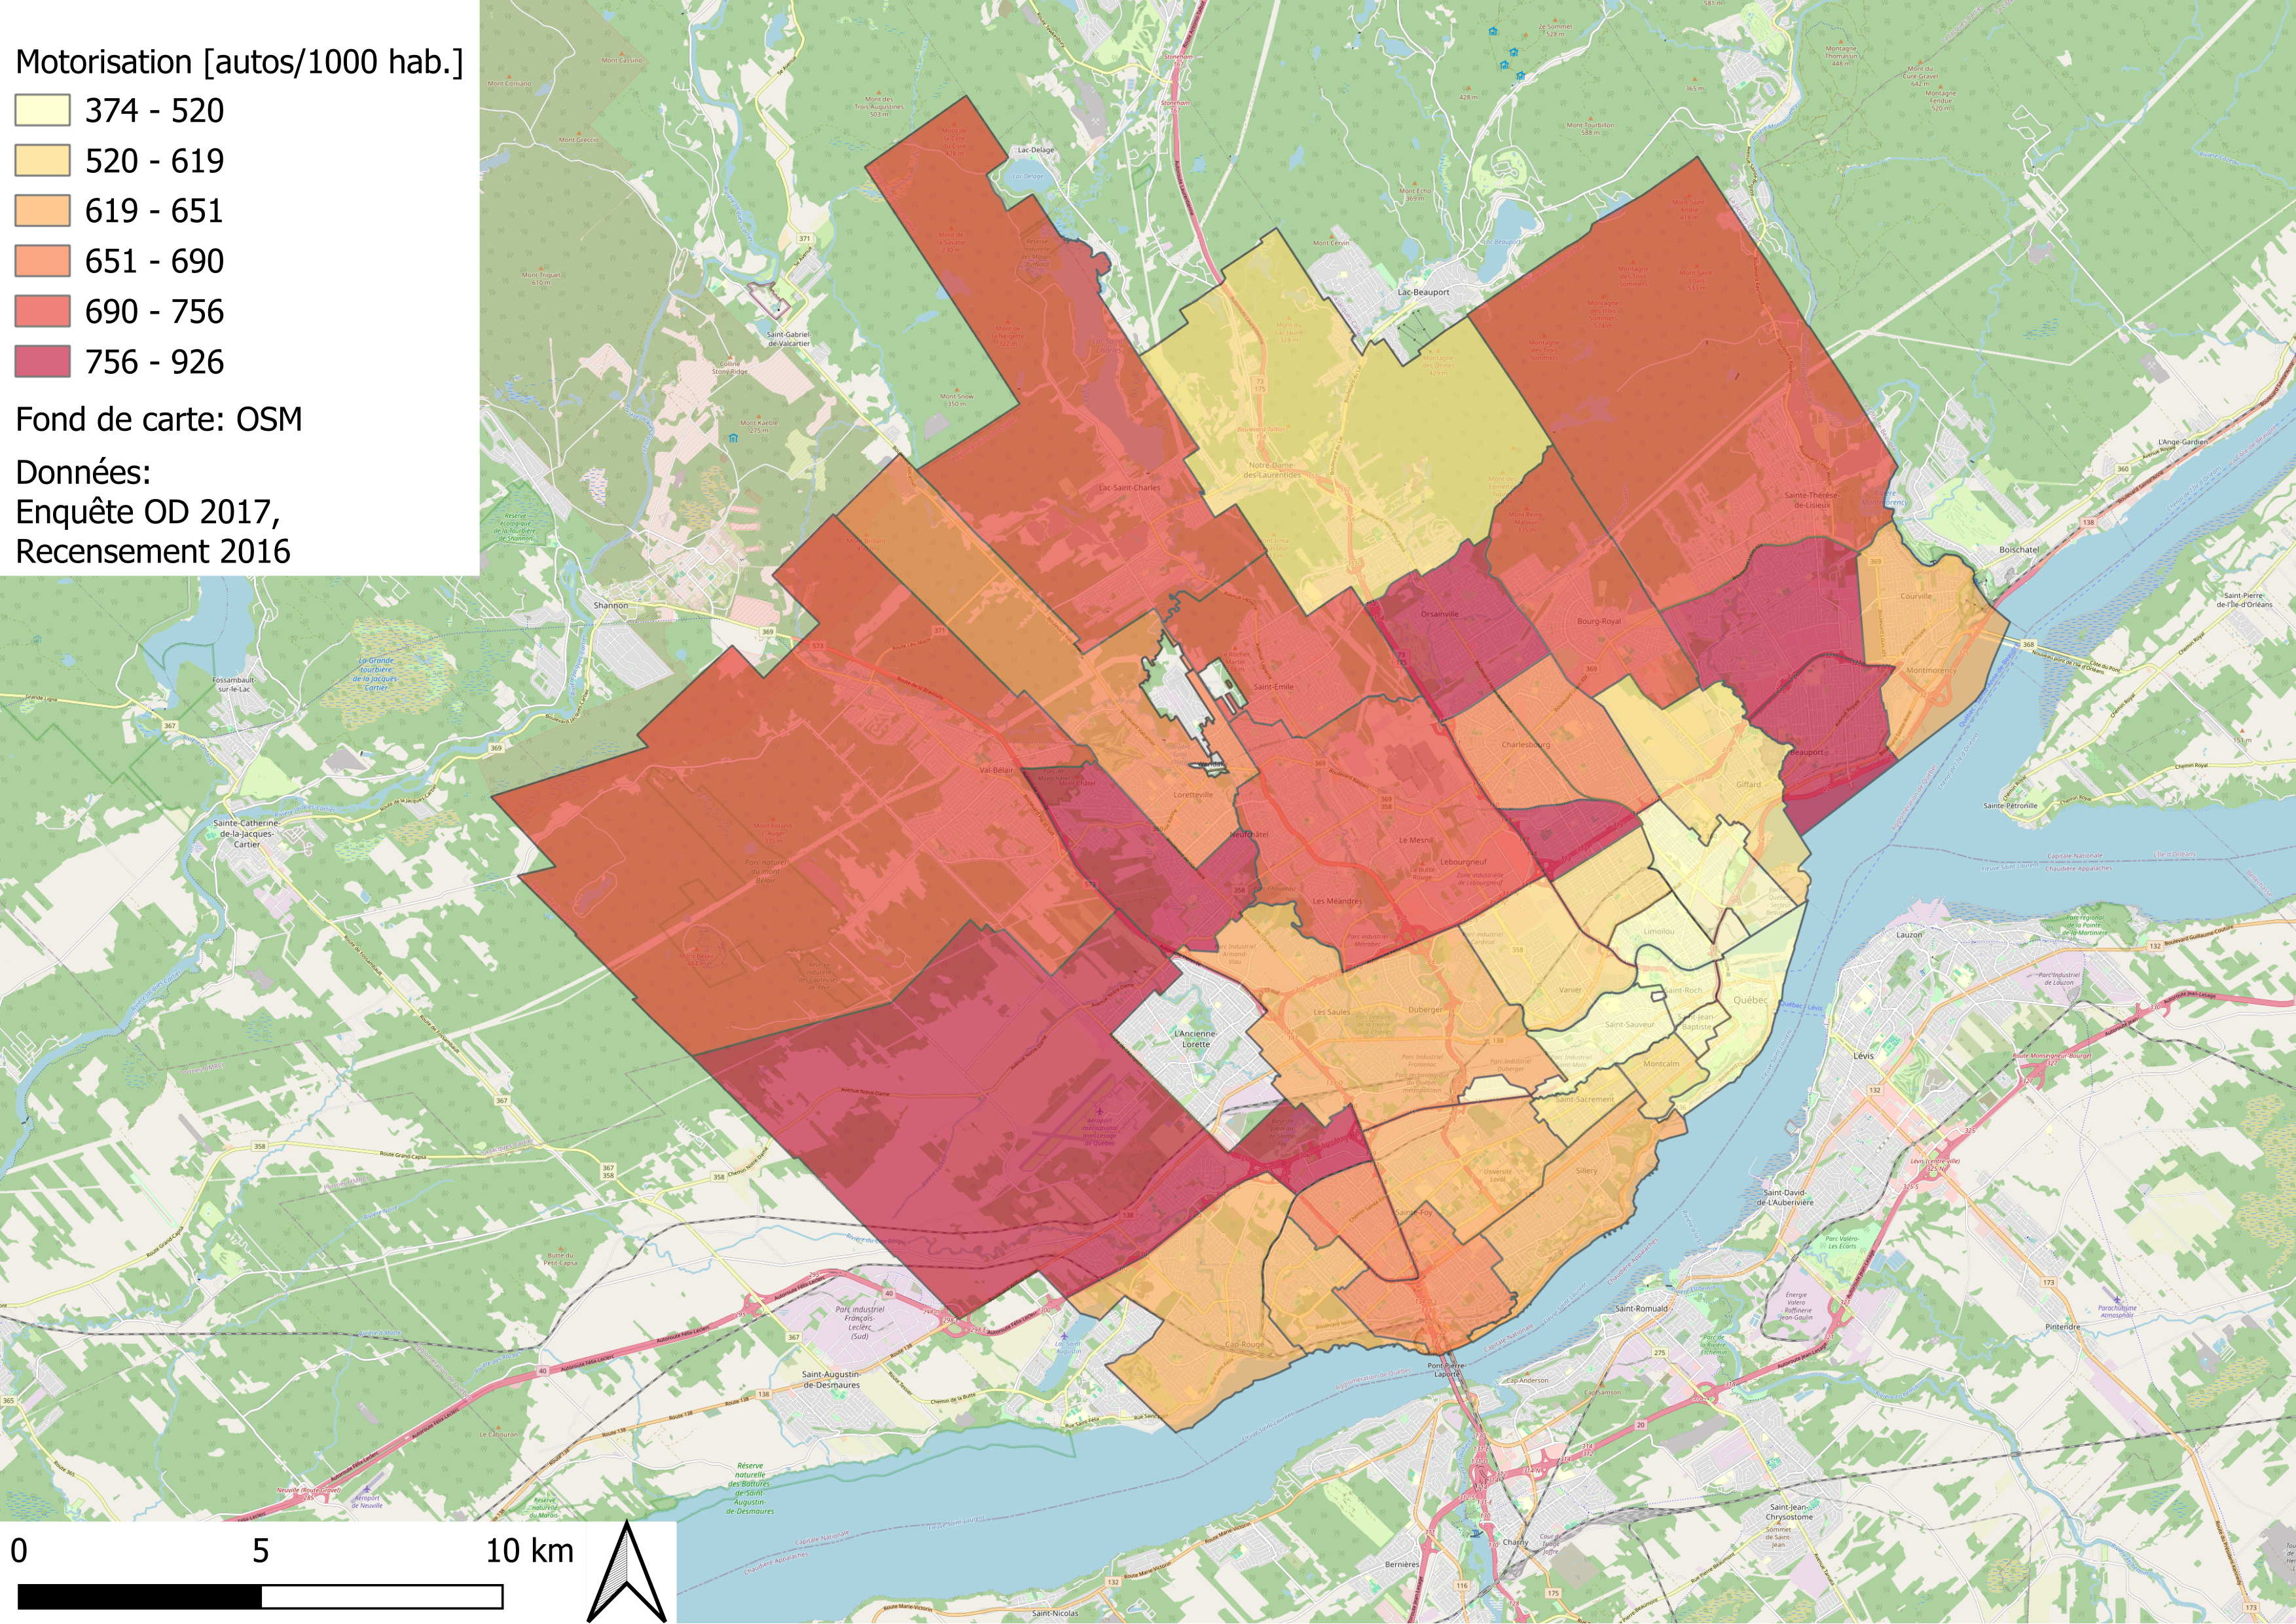
\includegraphics[width=0.65\linewidth]{images/motorisation-par-quartier.png}
    \caption{Motorisation selon les quartiers}
    \label{fig:motorisation-par-quartier}
\end{figure}
\FloatBarrier
Cependant, même en regardant le nombre de places de stationnement par logement, on constate des tendances contre-intuitives, puisque les quartier centraux paraissent mieux lotis que certains quartiers péri-urbains comme le montre la figure \ref{fig:stationnement-residentiel-par-quartier}. 
\begin{figure}[!h]
    \centering
    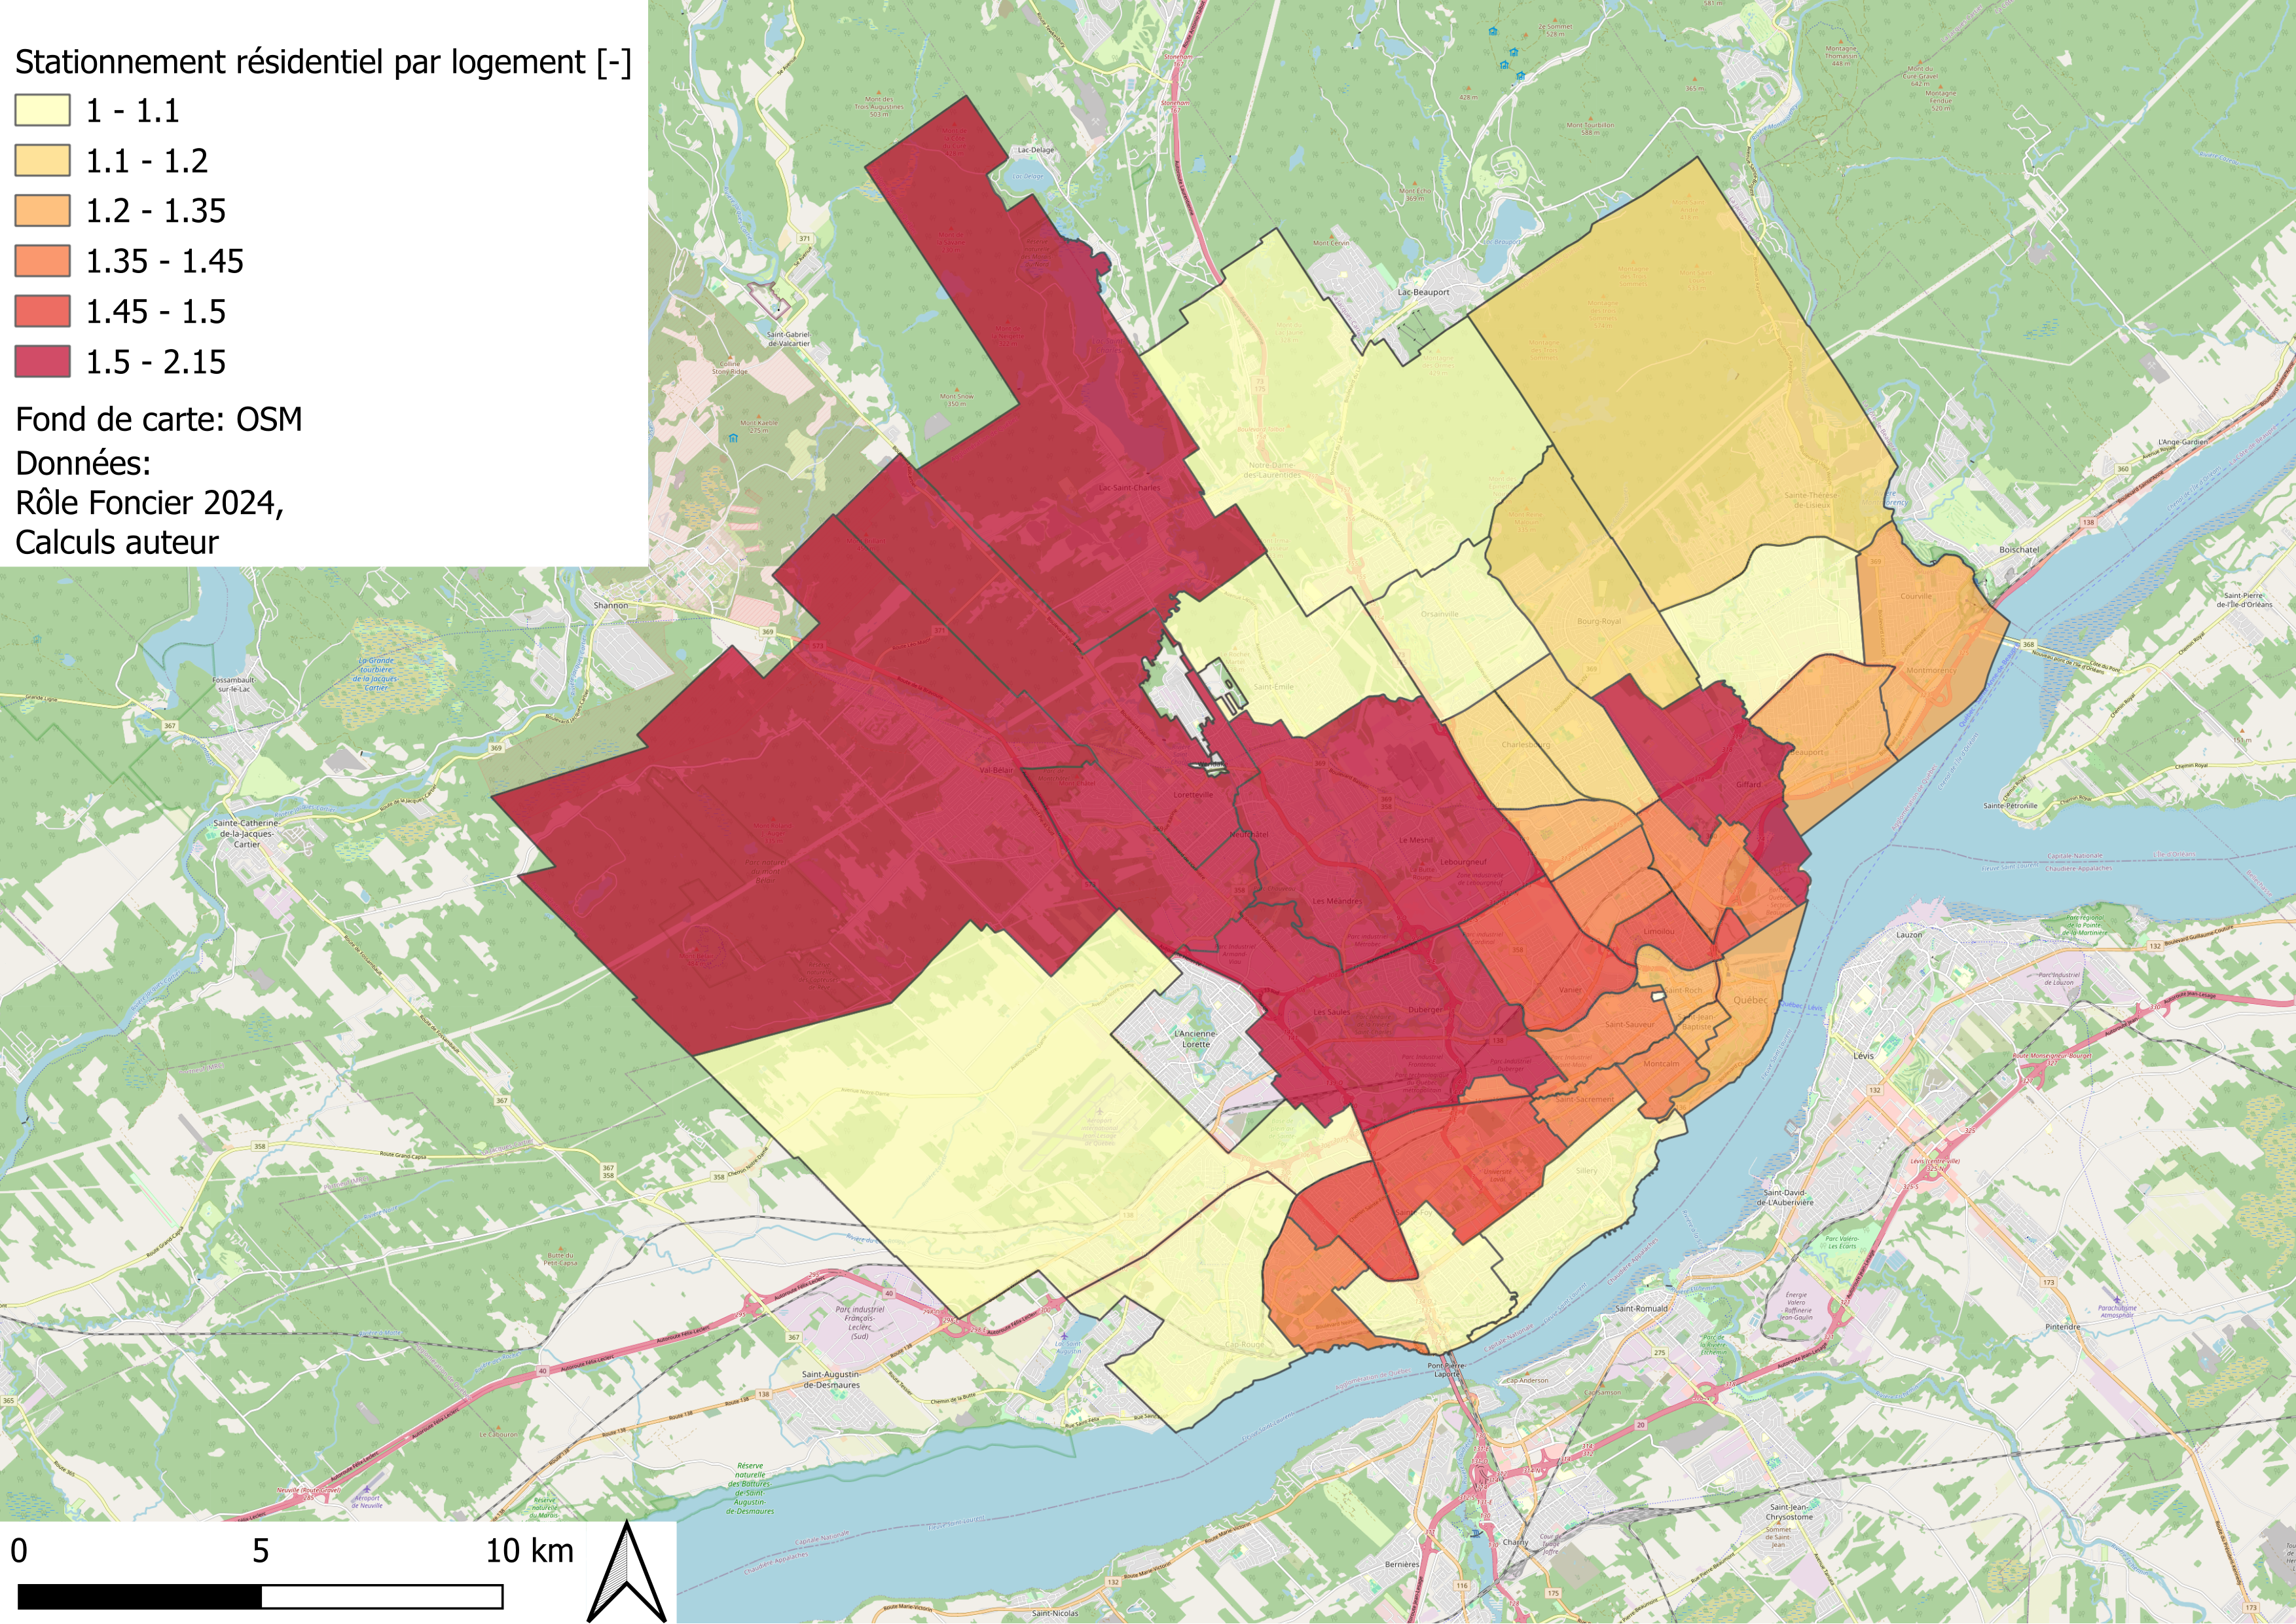
\includegraphics[width=0.65\linewidth]{images/stat-res-par-log.png}
    \caption{Stationnement résidentiel par logement}
    \label{fig:stationnement-residentiel-par-quartier}
\end{figure}
\FloatBarrier
On peut supposer qu'il y a deux dynamiques en jeu. Premièrement, les typologies de logement ne sont pas les même entre les quartiers centraux et les quartiers péri-urbains donc le nombre de places construites par rapport au minimum ne sera pas le même du fait de modèles d'affaires différents. Deuxièmement, les quartiers même à typologie similaire n'auront pas nécessairement des requis similaires donc le calcul actuel est potentiellement erroné.\par
Les profils d'accumulation véhicules peuvent aussi être donner une idée de l'utilisation de la capacité.Le parc total de stationnement complet peut être comparé à la population ou la capacité publique (c'est-à-dire autre que résidentielle) peut être comparé aux voitures hors-résidences, donnant potentiellement un meilleur portrait de la compétition aux destinations. La figure \ref{fig:PAV-cite-univ} montre le profile d'accumulation pour la Cité-Universitaire. Les lignes de capacité montrent la capacité réglementaire et une capacité ajustée. La capacité ajustée inclut les stationnement de la place Laurier et de certains stationnement du campus de l'université où les données manquaient.\par
\begin{figure}[h]
    \centering
    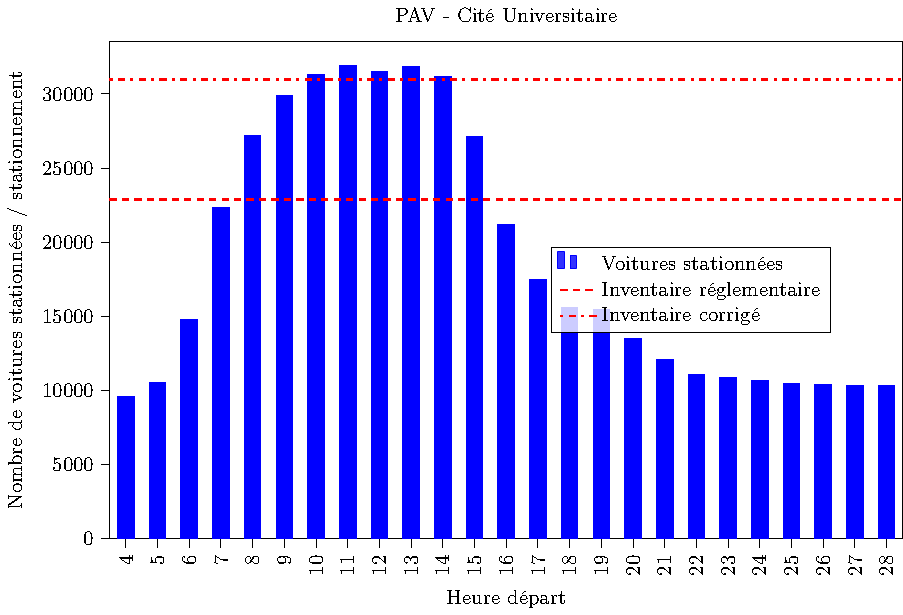
\includegraphics[width=1\linewidth]{figures/basic_PAV_CUNI.pdf}
    \caption{Profile d'accumulation de véhicules de la Cité Universitaire}
    \label{fig:PAV-cite-univ}
\end{figure}


Ce même exercice peut aussi être fait en isolant les voitures stationnées à la résidence ou dans un stationnement public. Les figure \ref{fig:pav-resi-cuni} et \ref{fig:pav-public-cuni} montrent l'accumulation de véhicules à la résidence contre la capacité résidentielle, et la même pour chose pour les places publiquement accessibles(autres que résidentielles). 
\begin{figure}[h]
    \centering
    \begin{subfigure}{1\textwidth}
        \centering
        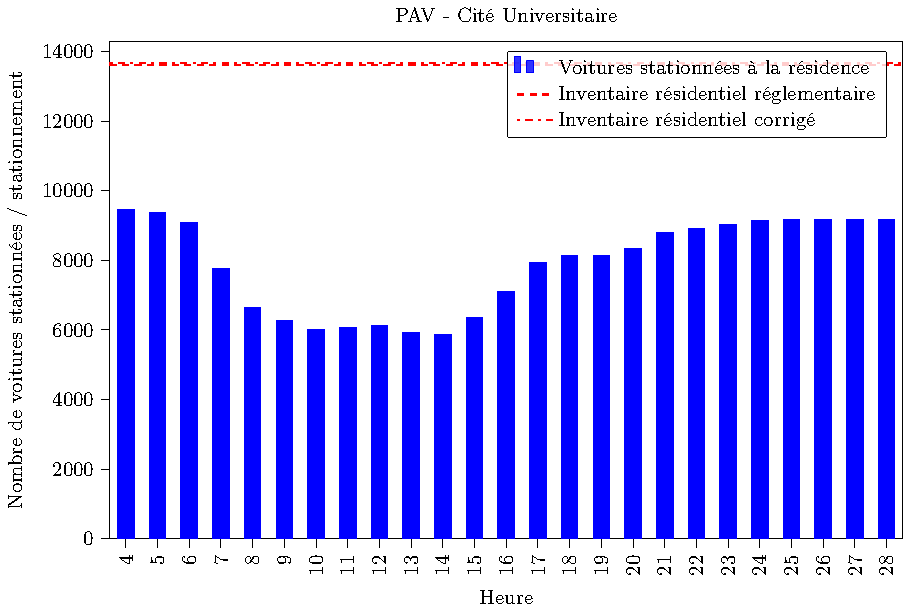
\includegraphics[width=0.8\linewidth]{figures/residential_PAV_CUNI.pdf}
        \caption{Résidentiel}\label{fig:pav-resi-cuni}
    \end{subfigure}
    \begin{subfigure}{1\textwidth}
        \centering
        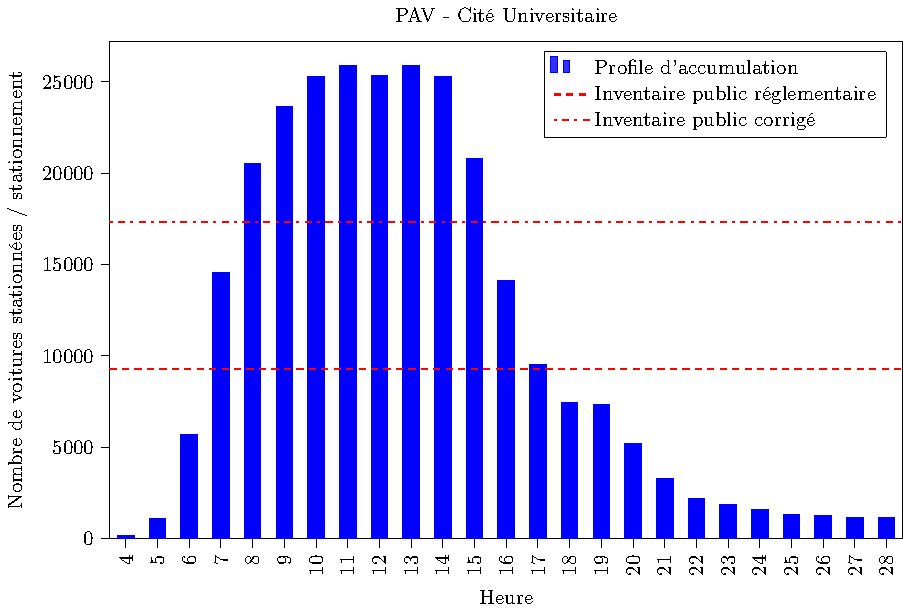
\includegraphics[width=0.8\linewidth]{figures/pub_PAV_CUNI.pdf}
        \caption{Destination}\label{fig:pav-public-cuni}
    \end{subfigure}
    \caption{Profiles d'accumulation de véhicules par clientèle}
    \label{fig:pav-by-clientele}
\end{figure}
On constate qu'il y a un grand manque à gagner dans les places de stationnement public. Des enjeux demeurent quant à la précision de l'inventaire et le fait de ne pas inclure le stationnement sur rue limite les possibilités d'interprétation.\par
La création de profils d'accumulation de personnes et de permis peuvent aussi être complétés pour la même zone et peut permettre d'inférer la consommation d'espace supplémentaire si chaque personne venait en automobile. La différentiation entre personnes et permis est mise en place pour comprendre quelles sont les personnes qui peuvent conduire qui ne viennent pas dans le quartier en voiture. Les figures \ref{fig:PAPERS-cuni} et \ref{fig:PAPERM-cuni} montrent comment la situation comment il y a beaucoup plus de personnes, détenteurs de permis ou non qui rentrent sur le territoire de la Cité-Universitaire. 
\begin{figure}[h]
    \centering
    \begin{subfigure}{1\textwidth}
        \centering
        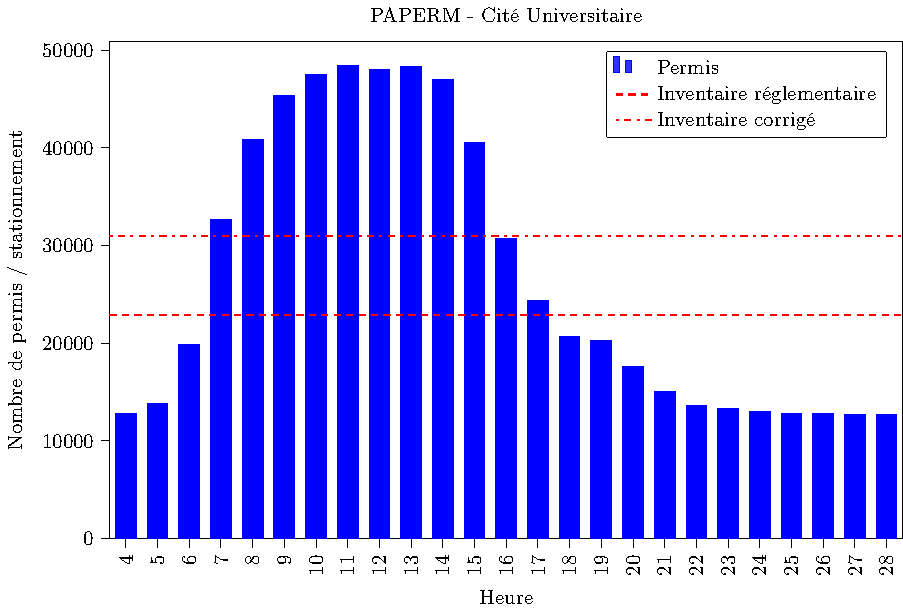
\includegraphics[width=0.8\linewidth]{figures/PAPERM_CUNI.pdf}
        \caption{Permis}\label{fig:PAPERM-cuni}
    \end{subfigure}
    \begin{subfigure}{1\textwidth}
        \centering
        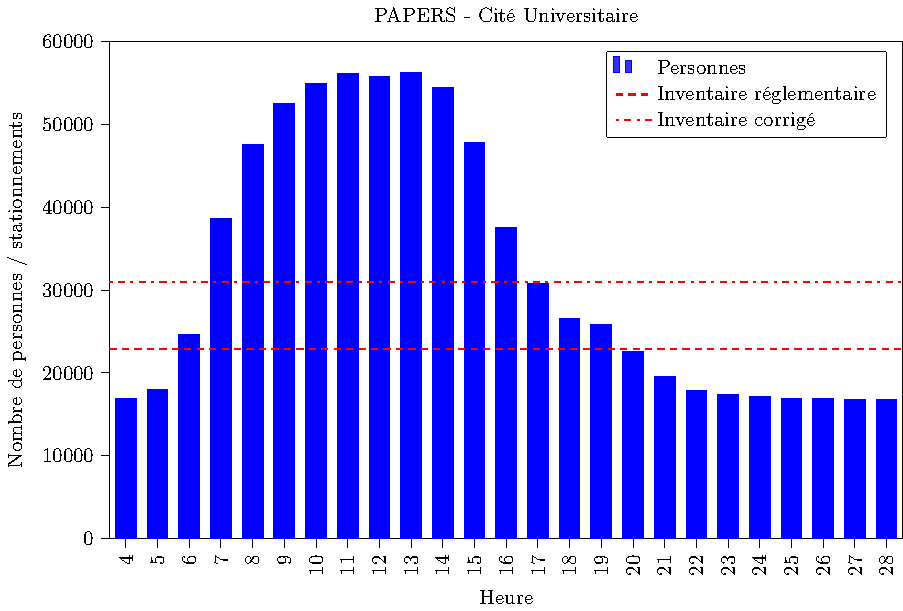
\includegraphics[width=0.8\linewidth]{figures/PAPERS_CUNI.pdf}
        \caption{Personnes}\label{fig:PAPERS-cuni}
    \end{subfigure}
    \caption{Profiles d'accumulation de personnes et permis}
    \label{fig:pap-cuni}
\end{figure}
La dynamique montrée pour la Cité-Universitaire n'est cependant pas la même que pour des quartiers plus excentrés qui sont plus des communautés dortoirs. La figure \ref{fig:pav-basic-orsa} montre le profile d'accumulation de base pour le quartier d'Orsainville qui se vide pendant la journée et où le stationnement résidentiel constitue 65\% de l'inventaire réglementaire (7882 places). Encore une fois, on constate que le stationnement prédit ne permet pas d'entreposer l'ensemble de la demande, menant à des questions sur la disponibilité du stationnement sur-rue et la fiabilité de l'inventaire. 
\begin{figure}
    \centering
    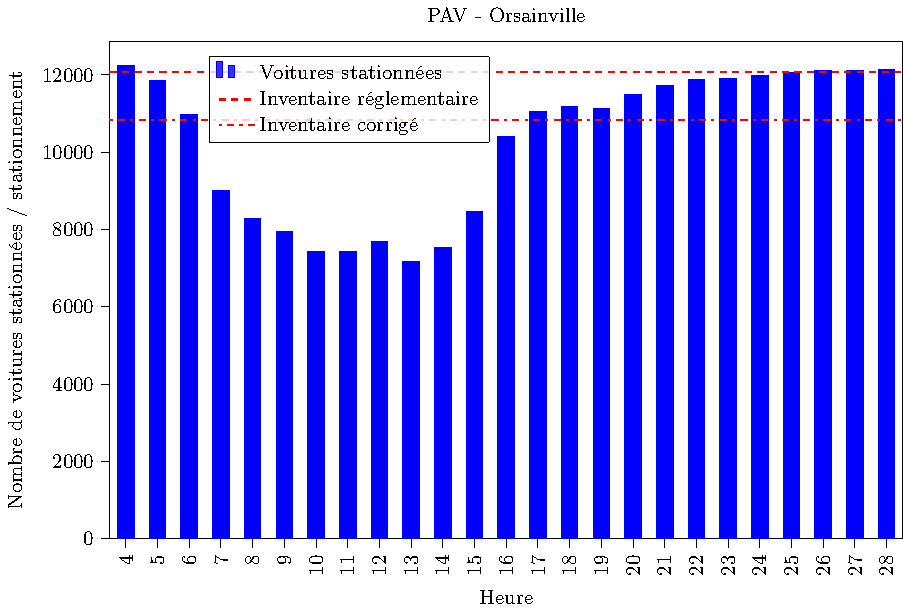
\includegraphics[width=0.75\linewidth]{figures/basic_PAV_ORSA.pdf}
    \caption{Profile d'accumulation d'Orsainville}
    \label{fig:pav-basic-orsa}
\end{figure}